\documentclass[11pt, a4paper]{article}
\usepackage[utf8]{inputenc}
\usepackage[margin=1in]{geometry} % Set 1-inch margins
\usepackage{graphicx}


\title{AA Final Exam}
\author{Andreas Riget Bagge \& Marcus Skjold Pedersen}
\date{2024-12-20}

\begin{document}
\maketitle

\section{Part 1}

\subsection{Task 1}
Our classic recursive MergeSort, \verb|TopDownMergeSort|, is largely based on \cite{Sedgewick_Wayne_2011}. It sorts an array by recursively divide it up, stopping at length 1. It then merges the subarrays back together pairwise, to sorted subarrays till the whole array is merged back together. The merging uses an auxiliary array, picking the lowest element from two subarrays one by one. In case of a tiebreak, we pick from the left subarray to ensure stability. The sum of compares for all merges is returned.

 We have tested for various cases for input-sizes and sortedness, regarding compares and correct sorting. We have tested on arrays with duplicate elements to ensure stability of the sort. For this we have made a \verb|TestData| class with an id-field and a value-field. We have tested \verb|Merge| also, focusing on cases where sub-arrays of even and differing sizes are merged.

\subsection{Task 2}

We see a very clear correlation between the number of comparisons and the  running times when varying the size of the array, see \ref{fig:t2p1}.
However, we ran many other experiments (See scripts.Task1.task2\_2) to investigate if by keeping the size constant and varying the number of comparisons by changing the ordering of the input array. These some aspects of these results were quirky, but broadly supported the hypothesis (more sorted input generally gives lower comparisons and running times than more randomized input).

\begin{figure}[h]
  \begin{center}
    % uncomment the line below to include the plot that you
    % automatically generated.
    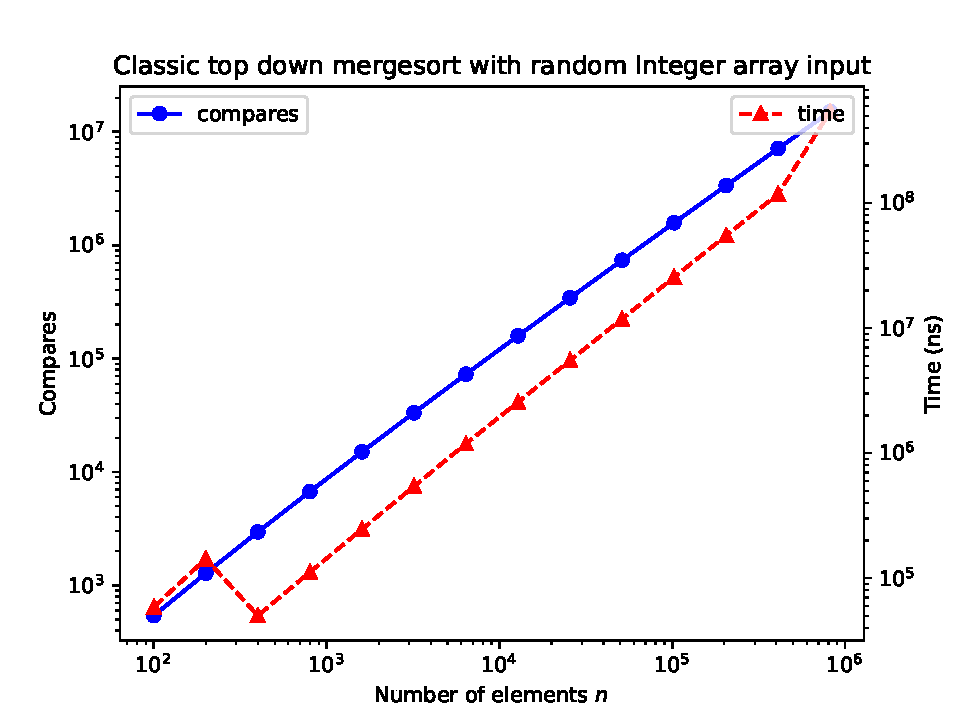
\includegraphics[width=\textwidth]{plot/t2p1.pdf}
    \caption{Comparing the increase in running time and comparisons.}
    \label{fig:t2p1}
  \end{center}
\end{figure}

\subsection{Task 3}

We have implemented a version of recursive mergesort with a base-case of insertion-sort for a parameter \verb|c| in \verb|TopDownMergeSortCutoff|. Rather than stopping the recursion for subarrays of size $\leq 1$, it stops at subarrays of sizes $c$ or less, and switches to Insertion-sort for the subarray instead.\footnote{As such, running the cutoff-variant (as well as the one in Task6) with c=1, corresponds to having no cutoff-value. However, to keeps tasks separate, we keep the two variants in different classes} We have implemented Insertion-sort in class \verb|Insertion-sort|, also inspired by \cite{Sedgewick_Wayne_2011}. 

We have tested that it handles cases where $c\leq 0$, throwing an error rather than looping indefinitely, and that it just performs insertionsort for $c\geq$ \verb|a.length|.

\subsection{Task 4}

We conducted an experiment to find the optimal cutoff value for $c$. We ran the algorithm with varying cutoff-values for varying array-sizes as seen in figure \ref{fig:runtimes}. The optimal $c$-value seems to lie around 10.

\begin{figure}[h]
  \begin{center}
    % uncomment the line below to include the plot that you
    % automatically generated.
    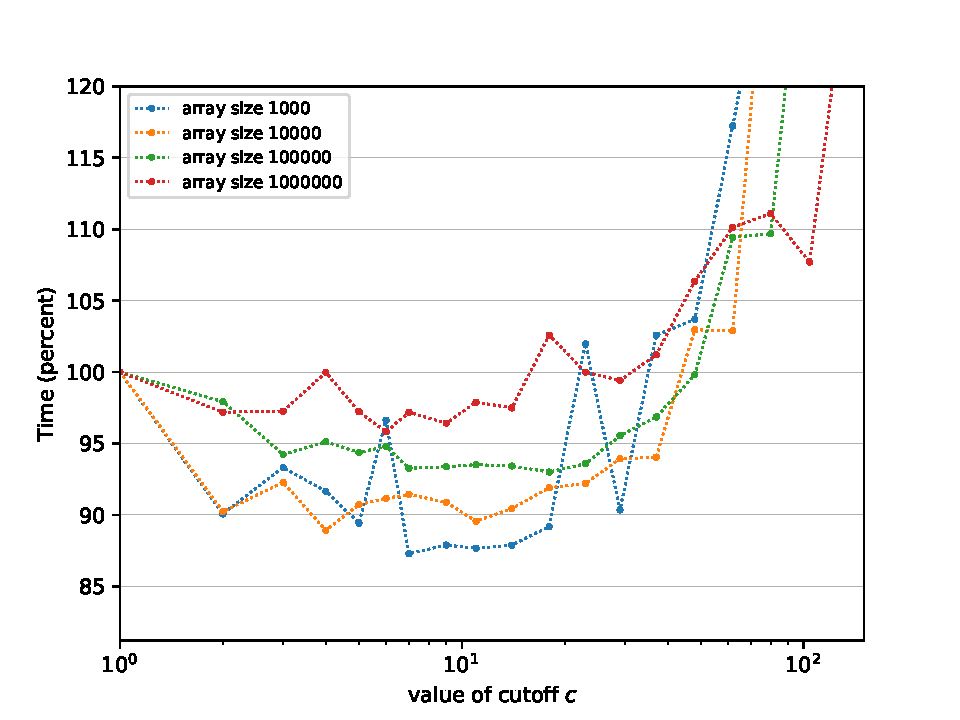
\includegraphics[width=\textwidth]{plot/t4p1.pdf}
    \caption{Running times for classic recursive mergesort with cutoff r relative to r = 1}
    \label{fig:runtimes}
  \end{center}
\end{figure}

\subsection{Task 5}

We have implemented an iterative version of merge sort using a stack in \verb|BottomUpMergeSort|. This implementation iterates through the input array, \verb|a|, adding each element as a run of length 1, to a stack of computed \textit{runs}. Then, if the next element in the stack has the same length as the newly computed run, they are merged. This is repeated till this condition no longer holds. 
When the end of \verb|a| has been reached, the stack of runs are merged together, one by one, top to bottom.

As the stack only holds runs of length $2^n, n\in \mathbf{N}$, with lengths of runs strictly decreasing, we have modeled the stack as a binary number, where a run of length $2^n$ is represented as the $n$'th bit being set. The position of runs in the stack can then be calculated based on this representation, simulating stack behavior.

 We have made tests to cover different cases of how the stack is filled and used for merges.

\subsection{Task 6}

We have made a variant of the algorithm in task 5, \verb|BottomUpMergeSortCutoff|, that makes new runs of size $c$ (using insertion sort) for a given integer $c\geq1$, rather than size 1. If less than $c$ elements remain in the array, insertion-sort is used on the remaining elements. 

This variant works similarly to the one in Task 5, however the stack is now scaled by $c$ when finding positions of runs, and also the array is iterated through in intervals of $c$, making runs with insertion-sort. Length $>c$ residues are computed with insertion-sort, and the final merge is then done similarly to Task 5.

We have implemented three variations of this algorithm and use by default the best performing of them. 

We have tested for special cases mentioned for the cutoff-variant in task 3. We have also made sure especially to test for cases where the last computed run is of length $<c$. 

\subsection{Task 7}

We ran an experiment similar to task 4 to determine an optimal value for $c$ for our iterative implementation. Following a similar approach we found that a $c$-value around 10 seems optimal.

\section{Part 2}

\subsection{Task 8}

We have implemented an adaptive and non-adaptive variant of Levelsort and BinomialSort. Both follow the run-stack-frame-work from Task5, with different merging policies. We have tested all implementations with respect to correctly sorting inputs, and with respect to compares. The latter, mainly to test their merging policies.

In our non-adaptive implementations, runs are created by using insertion-sort on the next c elements. In our adaptive variants, weakly increasing or strictly decreasing\footnote{using only \textit{strictly} decreasing runs ensures that their subsequent reversal is stable} sequences $>$ \verb|c| are used as a run. Locating the next run uses compares equal to the length of the run, except for the last run in the array, which uses 1 less compare. We have tested the adaptive variants with inputs of runs above and below c, and inputs with different amounts of runs.

\textbf{LevelSort:} Our Levelsort-implementations maintains a stack of computed runs accoording to their level. The level of a run is the level of its right boundary, based on the most significant bit in which the midpoints of the boundary-separated runs differ. As values of midpoints are strictly increasing left to right, two consecutive boundaries will never have the same level.

Our implementations merges runs by repeatedly computing the level of the boundary between the next two runs, \verb|L| and \verb|N|, from left to right. Then, as long as the level of \verb|L| is greater than the level of the top element in the stack, we merge \verb|L| with the top run, making the levels of the stack strictly increasing from top to bottom. Combined with the fact that consecutive runs differ in level, all levels in the stack are distinct. As such, we simulate the elements in the stack with a binary number, with the positions of set bits corresponding to the level of a run in the stack, the top of the stack being the least significant bit. The initial and last index of runs are saved in arrays, indexed by level. When the level of the top run in the stack exceeds the level of \verb|L|, \verb|N| becomes the new \verb|L|, and we find a new run \verb|N|. When no more runs can be found, the last run is mered with the runs in the stack, top to bottom.

We have tested different cases of the stack, such as inputs giving a run with the highest possible level compared to the stack, cases where no runs are merged before emptying the stack, and cases where parts of the stack are merged.

\textbf{BinomialSort:} Our implementations of BinomialSort maintains a stack of runs with monotnously increasing lengths, at least doubling pr. entry in the stack. As such, we keep track of the stack using a binary number, with arrays tracking the positions of runs. The two top runs are merged when this property is broken until it has been reestablished. We have tested BinomialSort similarly to Levelsort, mimicing different situations for the stack.



\subsection{Task 9}

We first ran our implementations on random inputs and inputs with minimum run sizes. Differences between adaptive and non-adaptive variants were minor here, indicating that adaptiveness plays a minor role in random input. For all algorithms the optimal $c$-value lied around 10-20.

We also tried input split into descending runs as seen in figure \ref{fig:descRuns}. Here the adaptive versions of our algorithms performed considerably better than the non-adaptive ones. This is expected, as the non-adaptive variants have to use insertion-sort on the reversed sequence, which is a worst case for insertion-sort. For our adaptive versions the c-value played a minor role, as long as it didn't exceed the length of runs in the input.

\begin{figure}[h]
  \begin{center}
    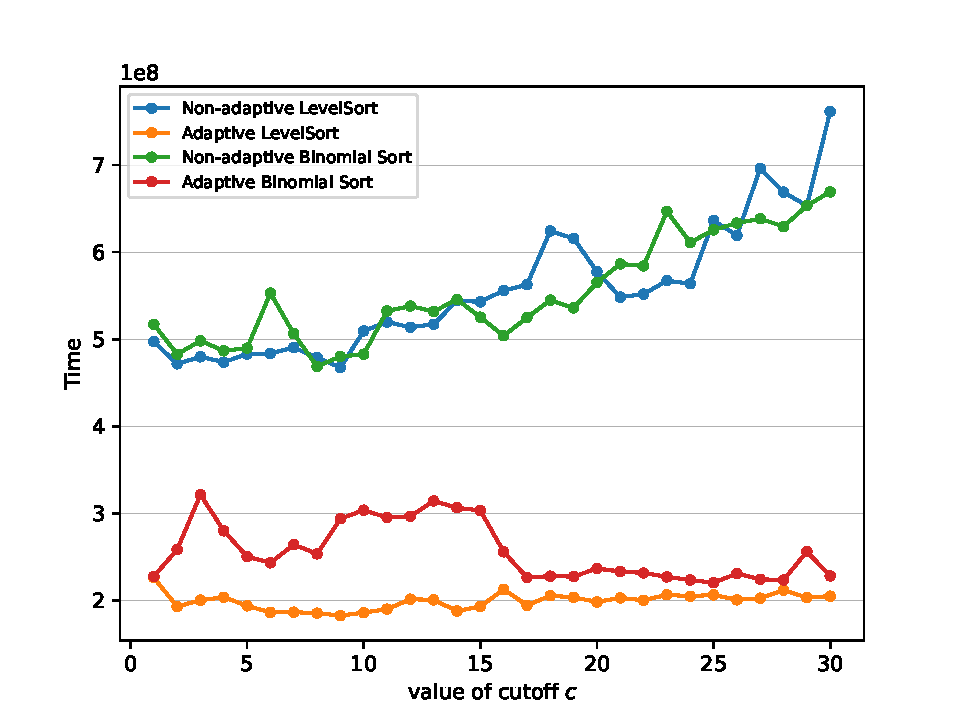
\includegraphics[width=\textwidth]{plot/t9more_runs_time_plot.pdf}
    \caption{Comparrison of adaptive vs. non-adaptive levelsort/binomialsort on input of descending runs}
    \label{fig:descRuns}
  \end{center}
\end{figure}


\subsection{Task 10}

We conducteda an experiment, comparing our (Adaptive) Levelsort and Implementationsort algorithms to our TopDown MergeSort implementation (with cutoff), our Insertion-sort-implementation and to \verb|Arrays.sort()|. 

We ran all the algorithms on random arrays of varying sizes.  Insertion-sort was clearly outperformed by the other algorithms. there was a general trend that \verb|Arrays.sort()| performed consistently better than the other implementations. This make sense as this method doesn't sort stably. The three other algorithms seemed to follow each other largely \textit{Task 9}.

We also tried to run the algorithms on input split up into runs as seen in figure \ref{fig:adaptComp}. Here, our implementations were, again outperformed by the library variant. However, they seemed to consistently perform better than recursive merge-sort. 

\begin{figure}[h]
  \begin{center}
    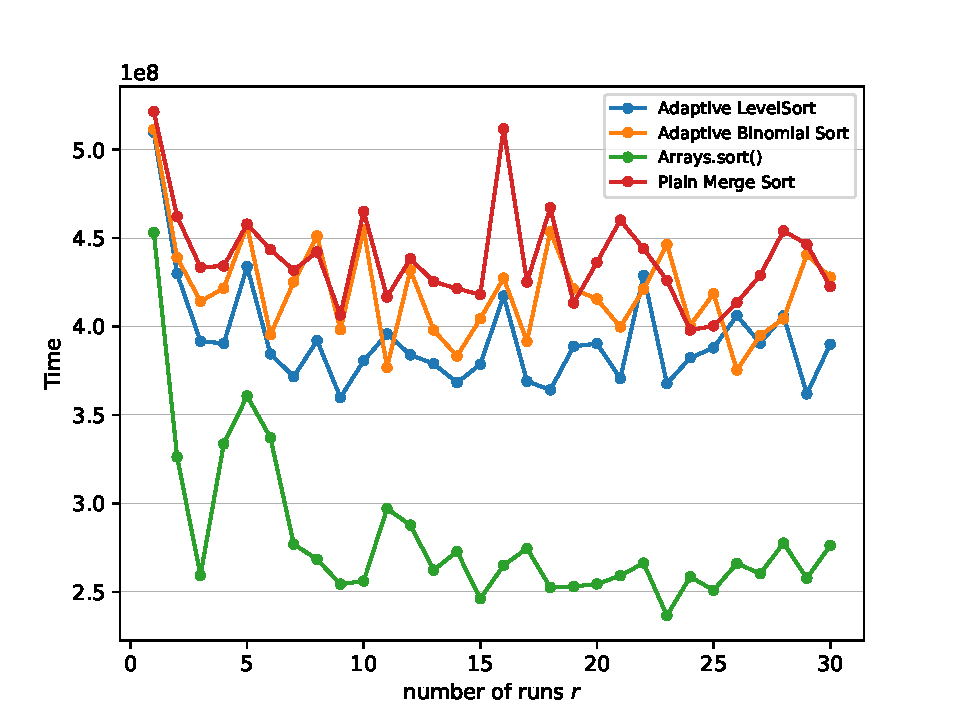
\includegraphics[width=\textwidth]{plot/t10runs_time_plot.pdf}
    \caption{Comparrison of LevelSort and BinomialSort to Arrays.sort() and TopDown MergeSort for input split into different amount of runs}
    \label{fig:adaptComp}
  \end{center}
\end{figure}




\section{Part 3}

For the parallel versions, we have copied the tests from the sequential versions, establishing that they give the same results. 
Further tests are for parallel-specific cases.

\subsection{Task 11}

Out parallel recursive merge sort (with sequential merge) is \texttt{Recursive\-MergeSort\-Parallel}. It has a cutoff value for switching to sequential sorting, and is implemented as \texttt{Recursive\-Task}'s in a \texttt{Fork\-Join\-Pool}.

\subsection{Task 12}

We see pretty clearly that the results improve up until the point where the ratio between
the size of the array and the cutoff parameter exceeds the number of available processors.
$n / c \leq available processors$.
This is in line with expectations: Parallelism should give improvement up until around the point where there are as many tasks ready as processors available.
This behavior is consistent across a range of array sizes for randomized sequences (see \ref{fig:t12p1}.
Results on our machines suggest that the speedup is stronger for higher array sizes.

\textbf{Potential speedup}: Set the parallel cutoff automatically relative to cores and n.

\textbf{Potential speedup}: Run sequential mergesort with an optimal cutoff (see Task 4).

The implementation is further tests with a repeated test to increase the chance of finding an undiscovered problematic interleaving.

\begin{figure}[h]
  \begin{center}
    % uncomment the line below to include the plot that you
    % automatically generated.
    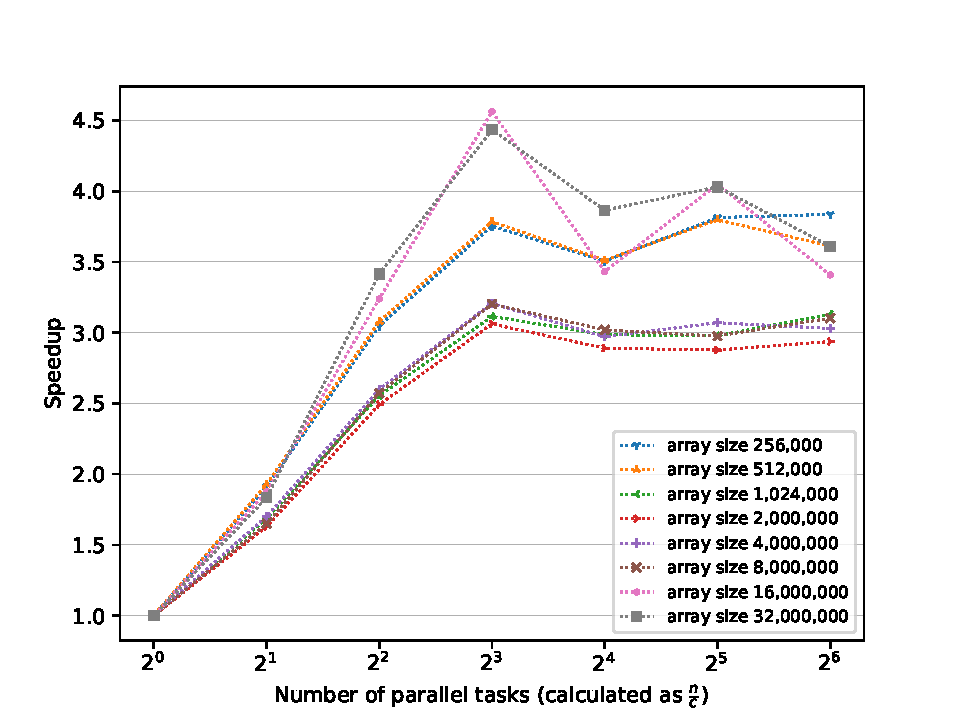
\includegraphics[width=\textwidth]{plot/t12p1.pdf}
    \caption{Measuring speedups of parallel merge sort (sequential merge) relative to running with no parallelism ($\frac{c}{n} = 1$)}
    \label{fig:t12p1}
  \end{center}
\end{figure}

\subsection{Task 13}

Our implementation has the signature MergeParallel.twoSequenceSelect(T[] in, int lo, int mid, int hi, int k).
Rather than use explicit sequences, as per the task description, we translate implicitly from a normal merge range, as it is used in our sequential implementation (See the JavaDocs for specifics).
The result given is a pair of integers: $i_a$, from which $i_b$ can be derived, as well as the comparison count. To use $i_a$ and $i_b$, they must be translated back into indexes in the input array ($i_a+lo, i_b+mid+1$)

\subsection{Task 14}

We have implemented a parallel version of merge using \texttt{twoSequenceSelect} to split the input merge sequence into $p$ parts.
The parts are created with as even size as possible, by rounding the next increment value (see lines 57, 63, 69 in \texttt{MergeParallel}).


\subsection{Task 15}

Our version of parallel merge sort using parallel merging can be used by specifying a $p$ parameter $> 1$ when calling the function.
We divide $p$ for each layer down the recursive tree we walk. This is to avoid generating wasteful amounts of parallel tasks, which would probably slow down the implementation.
If $p$ falls below 2, there is no point in using a parallel framework, and we switch to sequential merging.

\subsection{Task 16}

We see that in no case does our implementation beat \texttt{Arrays.parallelSort()}. However, we see that the performance of our implementation does improve as we allow for more threads to run in parallel.

\subsection{Task 17}

We have implemented the functionality for calculating the span. But we ran out of time while designing the experiment. We have written a test case showing that the correct span is returned in the test file and in the script file.

\newpage
\bibliographystyle{plain}
\bibliography{misc/cite}

\end{document}